


\section{Time series model}
\label{sec:model:TSMS}


% In this section we introduce some background concepts and the
% nomenclature which we will use later concerning TSMS. 

Measures and time series are the main objects of \acro{TSMS} and their
main characteristic is that they have a time attribute that requires a
coherent treatment. We describe the \acro{TSMS} nomenclature in three
parts: the data structure model, time series manipulation and
operation, and time series specific properties.



\subsection{Structure}


A \emph{time series} is a set of observations collected at specific
time instants. An observation may consist of a single attribute or of
multiple attributes collected at the same time instant.  Each pair of
time and observed values is called \emph{measure}. Then, a time series
is a relation of times with values described as a set of measures .



% Firstly we address time and value concepts and secondly we define formally
% measures and time series.


\subsubsection{Time}

Time, $t$, is an attribute that indicates order between measures. We define
$T$ as the \emph{time domain}. $T$ can be either a finite or an infinite set
and normally it will be a closed set. As an example for the time
domain $T$ we use the affinely extended real numbers $\Rb = \R \cup
\{+\infty,-\infty\}$ \cite{cantrell:extendedreal}.

The real numbers set is a metric space as it has a distance function
also called metric. Consequently, we can differentiate between time
instants (the elements of the set) and durations (the metric). In this
way, time can be defined as a coordinate system
\cite{iep:time-supplement,kopetz11:realtime} by noting time instants
as points in the real line, durations as segments of the real line,
and specifying a time instant as a reference time. Next, a time
definition is provided that allows to order events, measure events
duration, and position when events happen. This naive approximation
that avoids complex details of the time concept is enough for our
purposes.

\begin{definition}(Time)
  \label{def:model:temps}
  Let $t^i_i$ and $t^i_j$ be two \emph{time instants} with same $t^R$
  as \emph{reference time}, we define the \emph{quantity} or
  \emph{duration of time} $t^d$ as a value $t^d \in\Rb$ which measures
  the distance in time units between two time instants $t^d =
  d(t^i_i,t^i_j)$ where $d$ is the metric of the set $T$. When time
  instants are also real numbers $t^i_i , t^i_j \in \Rb$, then $t^d =
  t^i_i - t^i_j$.

  Let $T$ be the domain for time, we define a \emph{time instant} $i$
  as an element of the set $T$, $i \in T$. Following with the definition of
  a coordinate system and real numbers as time domain, let $t^{R}$ be
  a \emph{reference time instant}, then we define \emph{time instants}
  as a value $t^i \in\Rb$ that measures signed time distance from the
  \emph{reference time instant} $t^i= d(t^{R},i)$. $\square$
\end{definition}

Summarising, time instants position and order events, and between two
time instants there is a duration.  There are several time standards
\cite{allen:timescales} which specify how time duration must be
measured and how time instants positions must be noted.

Time standards deal with a similar concept of time coordinate system
which has been illustrated with real numbers. There is also a calendar
approach which define the time domain with names for the points in the
time line and with rules for time durations. Usually the aim of
calendars is to give a relation between time and Earth
rotation. Sometimes calendars are seen as essential parts of \acro{TSMS}
\cite{dreyer94}, however maps can be established between a time
coordinate system and a calendar system.



\subsubsection{Value}

Value, $v$, is an attribute that indicates the magnitude of measures. The
domain for values can be any data type, that is an object that belongs
to a determined set of values and that has operations associated.
This way valid examples for values are integers, real numbers,
strings, and more elaborated data structures such as arrays, lists, or
even other time series.

%For simplicity
In accordance to the time examples, for the value domain the
projectively extended real numbers $\R* = \R \cup \{\infty\}$ can be
used.  This example is for scalar values but can be extended to the
concept of multivalues $\R*^n$, which represent a collection of values
measured at the same time instant \cite{assfalg08:thesis}.




\subsubsection{Measure}

A measure associates the concepts of value measured in a particular
time instant.  In a general form, a definition for single values is
given and it can be extended to n-dimensional values.

\begin{definition}
  A \emph{measure} $m$ is defined as a tuple $m=(t,v)$ where $v$ is the
  value of the measure and $t$ is the time instant when the measure
  has been acquired.
\end{definition}

Let $m = (t,v)$ be a measure, $v$ is written as $V(m)$ and $t$ is
written as $T(m)$.


The time attribute defines the canonical order relation between
measures. There are two possible order relations, attending the case
when exists two measures with the same time but different value. Let
$m = (t_m, v_m)$ and $n = (t_n, v_n)$ be two measures.  (i) A
\emph{partial order} is obtained when both measures are equal as a
whole, $m \geq n$ if and only if $t_m > t_n$ or $(t_m, v_m) = (t_n,
v_n)$, as then two measures are not ordered when only $t_m =
t_n$. (ii) A \emph{total order} is obtained when both measures are
equal only considering the time attribute, $m\geq n$ if and only if
$t_m\geq t_n$, as then measures are always ordered.  We also call
\emph{temporal order} to the total order.



\subsubsection{Time series}

Time series are sets of measures of the same phenomena that are
ordered in time.  Sometimes they are also called time sequences
\cite{last:hetland}.


\begin{definition}
  \label{def:model:timeseries}
  A \emph{time series} $S$ is a set of measures $S = \{m_0, \ldots,
  m_k\}$ without repeated time values $\forall i,j:i\neq j: T(m_i)\neq
  T(m_j)$.
\end{definition}

As there are no repeated time values, measures in a time series have a
total order.

Given a time series $S$, its cardinality is noted as $|S|=k+1$.  A
time series without measures is the empty time series,
$S_\emptyset=\emptyset=\{\}$, and has zero cardinality,
$|S_\emptyset|=0$.  Observe that, because measures in $S$ are of the
same phenomena, the type of $S$ values is homogeneous.



A time series can record more than one phenomena if they share the
time instants of acquisition. Then it is a \emph{multivalued time
series}, which can be expressed by two forms. Let $S = \{m_0, \ldots,
m_k\}$ be a time series, in one form we write measures as
$m=(t,(v_1,v_2,\ldots,v_n))$, that is the value has domain $\R*^n$; in
the other form we write measures directly as
$m=(t,v_1,v_2,\ldots,v_n)$.




\subsection{Operations}
\label{sec:model:operations}

Time series have a time attribute that must be manipulated
coherently. Owing to this time attribute, the behaviour of a time
series can be handled on three ways:  set operations including
relational ones,  sequence operations, and  temporal function
operations that manipulate a time series considering it is a
representation for a continuous function. Next a brief description of
most important ones is given.


These time series manipulations are defined abstractly for any time
series having the structure of Definition \ref{def:model:timeseries}.
In the same way as the relational model for operations, definitions
evaluate algebra and logic concepts for data but do not evaluate the
semantics of manipulations. That is, when given a particular context
for a time series manipulation it has to be decided whether the
algebra is meaningful or cannot be applied, for example an addition of
values in two different units could be semantically erroneous.


\subsubsection{Set operations}

We describe how common set operators can be applied to time series. We
rely on how the relational model of DBMS describes operations based on
set algebra \cite{date:introduction}.


In a time series the measures have a total order.  As a time series is
a finite set, if it is not empty it has a maximum and a minimum.  Let
$S$ be a time series and $n\in S$ be a measure, the time series'
\emph{maximum} is $n=\max(S)$ if and only if $\forall m \in S: n \geq
m $.  We extend the maximum definition with a supremum one as for
extended real numbers the supremum is defined even when a set is
empty, $\sup(\emptyset)=-\infty$ \cite{cantrell:extendedreal}. So
applying this property we can say $n=\sup(S)$ is the \emph{supremum}
of the time series where $n=\max(S)$ when defined and
$n=(-\infty,\infty)$ otherwise; note that $V(n)=\infty$ is an
indefinite value.  Dually, we can define \emph{minimum} $\min(S)$ and
\emph{infimum} $\inf(S)$.


In time series binary set operations, the measures can have the
two possible order relations: total and partial. Consequently, this two
possible order relations of measures induces two operation definitions
for some set operators.  Mainly it induces two membership operations
and so to all operations based on it. 


The \emph{membership} defines when one measure belongs to a time
series. Considering the partial order of measures, the set
membership operation applies. Let $S$ be a time series and $m$ a
measure, the \emph{membership} is denoted $m \in S$. Considering the
temporal order of measures, we define the \emph{temporal membership}
as $m \inst S$ when $\exists m_a \in S : T(m) = T(m_a)$.  Let $S_1$
and $S_2$ be two time series, from membership operations we could
define \emph{inclusion} $S_1\subseteq S_2$ and \emph{temporal
  inclusion} $S_1\subseteqt S_2$.


The \emph{union} of two sets is a set containing elements from both
sets. Plain set union operation can not be applied directly as the
resulting time series could have repeated time values.  So we define a
non commutative operation and a commutative temporal operation. The
union requires both time series to have the same structure and type as
happens with union operation in relational \acro{DBMS}
\cite{date:introduction}. %
Let $S_1$ and $S_2$ be two time series. The \emph{union} of both is a
time series $S_1 \cup S_2$ with all measures of $S_1$ and those not
repeated at $S_2$: $S_1 \cup S_2 = \{m^1 \in S_1 \vee m^2 \in S_2 |
m^2 \notinst S_1 \}$. The \emph{temporal union} of both is a time
series $S_1 \cupt S_2$ with all measures from $S_1$ and $S_2$
excluding those that only share the time attribute: $S_1 \cupt S_2 =
\{ m^1 \in S_1 \vee m^2 \in S_2 | m^1 \notinst S_2 \vee m^1 \in S_2,
m^2 \notinst S_1 \}$.

\begin{figure}
  \centering
  %\def\escala{0.9}

\def\nodeA{node [above left=0.5cm and 0.1cm] {$(1,1)$} node [below left=0.5cm and 0.1cm] {$(5,1)$}}
\def\nodeB{node [above right=0.5cm and 0.1cm] {$(2,2)$} node [below right=0.5cm and 0.1cm] {$(6,2)$}}
\def\nodeT{node [above=0.1cm] {$(4,0)$} node [left=0.4cm] {$(3,1)$} node [right=0.4cm] {$(3,2)$}}
% Definition of circles
\def\firstcircle{(0,0) circle (1.5cm)}
\def\secondcircle{(0:2cm) circle (1.5cm)}
\def\thirdcircle{(0:1cm) circle (1.11cm)}

\colorlet{circle edge}{blue!50}
\colorlet{circle area}{blue!20}

\tikzset{
  filled/.style={fill=circle area, draw=circle edge, thick},
  outline/.style={draw=circle edge, thick},
  every node/.style={transform shape}
}

%\setlength{\parskip}{5mm}






%Set A or B
\begin{tikzpicture}[scale=\escala]
  \draw[filled] \firstcircle \nodeA;
    \begin{scope}
        \clip \secondcircle;
        \draw[filled, even odd rule] \firstcircle \nodeA
                                 \secondcircle 
                                 \thirdcircle;
   \end{scope}
    \draw[outline] \firstcircle
                   \secondcircle \nodeB
                   \thirdcircle \nodeT;

   \node[anchor=south] at (current bounding box.north) {$S_1 \cup S_2$};
\end{tikzpicture}
%Set temporal A or B
\begin{tikzpicture}[scale=\escala]
    \draw[filled, even odd rule] \firstcircle \nodeA
                                 \secondcircle \nodeB
                                 \thirdcircle \nodeT;
    \node[anchor=south] at (current bounding box.north) {$S_1 \cup^t S_2$};
\end{tikzpicture}






%%% Local Variables:
%%% TeX-master: "../main"
%%% ispell-local-dictionary: "british"
%%% End:

  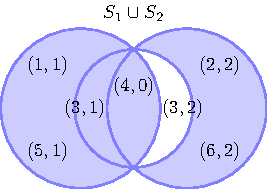
\includegraphics{fig_model_venn.pdf}
  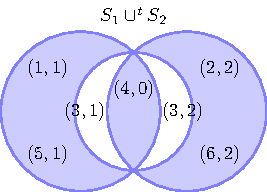
\includegraphics{fig_model_venn2.pdf}
  \caption{Venn diagrams examples for set and temporal set union
    operation of \acro{TSMS}}
  \label{fig:model:venn}
\end{figure}


\begin{example}\label{ex:model:s1s2}
  Let $S_1=\{(1,1),(3,1),(4,0),(5,1)\}$ and $S_2 = \allowbreak
  \{\allowbreak (2,\allowbreak 2),\allowbreak (3,2),(4,0),(6,2)\}$ be
  two time series. The union from first and second results $S_1 \cup
  S_2 = \{(1,1),\allowbreak (2,2),\allowbreak (3,1),\allowbreak (4,
  0),\allowbreak (5,1),\allowbreak (6,2)\}$. The temporal union from
  both results $S_1 \cupt S_2 = S_2 \cupt S_1 =
  \{(1,1),(2,2),(4,0),(5,1),\allowbreak (6,2)\}$. %
  Venn diagrams for both cases are shown in
  Figure~\ref{fig:model:venn}, where the coloured area is the
  resulting time series. For each, the central intersecting area
  indicates measures that share time and value attributes, as instance
  $(2,0)$. The central left area are measures from $S_1$ that only
  share the time attribute with a measure from $S_2$, as instance
  $(3,1)$. Dually the central right area contains $(3,2)$. The left
  and right outer areas are the remaining measures.
 \end{example}




The \emph{difference} of two sets is a set containing all elements
from first not contained in second. Like union, the difference
requires both time series to have the same structure. %
Let $S_1$ and $S_2$ be two time series, the \emph{difference} of first
and second is a time series $S_1 - S_2$ with all measures of $S_1$ not
belonging to $S_2$: $S_1 - S_2 = \{ m \in S_1 | m \notin S_2
\}$. The \emph{temporal difference} of first and second is a time
series $S_1 - S_2$ with all measures of $S_1$ not temporal belonging
to $S_2$: $S_1 -^t S_2 = \{ m \in S_1 | m \notinst S_2 \}$.


Based on union and difference we can define \emph{intersection} $S_1\cap
S_2 \equiv S_1 - (S_1 - S_2)$ and \emph{symmetric difference} $S_1 \ominus
S_2 \equiv (S_1 - S_2) \cup (S_2 - S_1)$ operations as well as its
temporal dual operations.


Relational DBMS extend these set operators with specific ones like
projection, selection, rename, product and join. These operators can
be also used for time series. As example the definition of join
operation is given.


The \emph{join} of two time series is the grouping of pairs that share
the same time attribute in both.  Let $S_1$ i $S_2$ be two time series,
the \emph{join} of both time series $S_1 \join S_2$ is a multivalued
time series $S_1 \join S_2 = \{ (t,v_1,v_2) | (t_1,v_1) \in S_1 \wedge
(t_2,v_2) \in S_2 \wedge t=t_1=t_2 \}$.


\acro{DBMS} need computational operations to be able to compute with
the elements contained in time series. In relational \acro{DBMS} these
operators are extend, aggregate and summarise
\cite{date:introduction}. For time series, we define a more general
equivalent computational operators map and fold.


Map applies a function to each measure of a time series.  Let $S$ be a
time series and $f^m$ a function over a measure where $f^m:m_a\mapsto
m_r$, the \emph{map} of $f^m$ to $S$ is a time series $\map(S,f^m) =
\{\forall m_i\in S : f^m(m_i) \}$.

Fold recursively combines every measures of a time series.  Let
$S=\{m_0, \dotsc, m_k\}$ and $S_i$ be two time series, and $f^f$ a
function over a time series $S_a$ and a measure $m_b$ resulting in a
time series $S_r$, $f^f: S_a \times m_b \mapsto S_r$. The \emph{fold}
of $S$ by $f^f$ with initial value $S_i$ is a time series
$\fold(S,S_i,f^f) = f^f(\dots( f^f(f^f(f^f(S_i,m_0),\allowbreak
m_1),\allowbreak m_2 )\dots),\allowbreak m_k)$.


A simplified fold operation is \emph{aggregate} which is used for
combining a time series into one measure, normally it is used to
compute aggregate statistics.  Let $S$ be a time series, $m_i$ a
measure, and $f^a$ a function over two measures where $f^a: m_a \times
m_b \mapsto m_r$.  Based on fold operation \emph{aggregate} can be
defined as: $\agg(S,m_i,f^a) \equiv \fold(S,\{m_i\},f')$ where $f':
\{m_i\} \times m \mapsto \{f^a(m_i,m)\}$.

%A more generic version of fold is a fold considering order. 
In the previous fold the measures are computed in random order,
however in some computational operations it is necessary to define the
order, especially when $f^f$ is not commutative. We define a
\emph{fold with order}, $\orderfold$, as an extension of fold with a
function $o$ that selects measures in order where $o: S_a \mapsto m_r$
\[
 \orderfold(S,S_i,f^f,o) =
  \begin{cases}
    S_i  \text{ if } |S|=0, \\
    \orderfold(S_o,f^f(S_i,m_o),f^f,o)  \text{ otrw.}
  \end{cases}
\]
where $m_o = o(S)$ and $S_o = S - \{m_o\}$.


Finally, we describe how \emph{binary computational} operations can be
defined for two time series in order to operate with their value
attributes.  First it is required to join the two time series and then
apply computational operations. Let $S_1$ and $S_2$ be two time series
and \emph{op} be a binary operation on the value domain, that is for
two values $v_1$ and $v_2$ it computes a new value $\operatorname{op}:
v_1 + v_2 \mapsto v'$. The operator \emph{op} can be applied to both
time series as: $\operatorname{op}: S_1 \times S_2 \mapsto S'$ where
$S' = \map(S_1 \join S_2, (t,v_1,v_1)\mapsto(t,v_1 \operatorname{op}
v_2))$.

For example, we can apply real numbers binary operations such as sum,
$S_1 + S_2$, or division, $S_1 / S_2$. It must be noted that join
requires both time series to have exactly the same time
attribute. When time series diverge too much then temporal function
operations can be applied to fit the time instants to what is
required.





\subsubsection{Sequence operations}

Sequence operations manipulate time series considering measures as
being totally ordered. Then three basic operations can be defined:
interval, successor and concatenation.


The \emph{interval} $(t_i,t_f)$, where $t_i$ and $t_f$ are two time
instants, over a time series $S$ is a time subseries between the two
time instants $S(t_i,t_f) \subseteq S$. A similar interval concept
is used by \cite{last:hetland}. The open interval is defined as
$S(t_i,t_f)=\{m\in S | t_i<T(m)<t_f\}$. Other intervals can be
defined: closed $S[t_i,t_f]$, left-open $S(t_i,t_f]$, and right-open
$S[t_i,t_f)$.

The time order in time series also implies the sequence concept of
\emph{successor} and \emph{predecessor}.  Let $S=\{m_0, \ldots, m_k\}$
be a time series and $m_S\in S$ and $m_a$ be two measures. We say
$m_S=\nex_S(m_a)$ is the \emph{next} measure to $m_a$ in $S$ if and
only if $m_S=\inf(S(T(m_a),+\infty])$.  We say $m_S=\prev_S(m_a)$ is
the \emph{previous} measure to $m_a$ in $S$ if and only if
$m_S=\sup(S[-\infty,T(m_a)))$. %
Infinite measures are obtained when next and previous are applied to
supremum and infimum measure respectively: $\nex_S(\sup
S)=(+\infty,\infty)$ and $\prev_S(\inf S)=(-\infty,\infty)$.



\emph{Concatenation} comprises the measures of the first time series
followed in time order by the measures of the second. It is similar to
union for sets but considering the sequence interval. The
concatenation requires both time series to have the same structure as
seen with union operation.  Let $S_1$ and $S_2$ be two time series,
the concatenation of both $S_1 || S_2$ is a time series $S$ containing
all measures of $S_1$ and those of $S_2$ that not intersect in the
time interval of $S_1$.  $S_1 || S_2 = S_1 \cup ( S_2 - S_2[t_1,t_2]
)$ where $t_1=T(\inf S_1)$ and $t_2=T(\sup S_1)$.



\subsubsection{Temporal function operations}
\label{sec:model:tfunc}

A time series is a discrete representation of a continuous function,
more precisely a temporal continuous function as time is the function
domain. Operations that manipulate time series according to this
temporal function nature can be defined.

The \emph{graph of a function} allows to obtain and interpret the
continuous nature of a time series, when the domain of time and value
attributes can be plotted then the graph is equivalent to a graphical
representation.  Let $S$ be a time series and $T$ the time domain, the
\emph{graph} of the time series is a set of ordered pairs $\graph S =
\{ (t,S(t)) | t\in T \}$ where $S(t)$ is a temporal representation
function for the time series.

The \emph{temporal representation function} $S(t)$ is a continuous
function along variable $t$ in the domain of time and the target in
the domain of values. $S(t)$ can be obtained by various methods, so
there are several possible temporal representation functions. In all
temporal function operations a superscript $r$ indicates the name $r$
of the representation method used, as instance $S(t)^r$ is the
representation function using method $r$. We exemplify the
representation functions using two methods $r$ based on impulse and
constant piecewise functions.


\begin{definition}
  \emph{Dirac delta} (\dd) is a method of representation based on the
  Dirac delta function. It is an impulse train function that is zero
  everywhere except at zero.  Let $S$ be a time series we define
  $S(t)^\dd$ as the \emph{\dd{} representation function}
\[
    \forall m \in S: S(t)^\dd
    =  \begin{cases}
      V(m) & \text{if }  t=T(m) \\
      0 & \text{otherwise}
    \end{cases}
\]
\end{definition}

\begin{definition}
  \emph{Zero-order hold everted} (\zohe{}) is a method of
  representation based on the \emph{zero-order hold} signal
  reconstruction methods. It is a piecewise constant function that has
  left-continuous step functions.  Let $S$ be a time series we define
  $S(t)^\zohe$ as the \emph{\zohe{} representation function}, $\forall
  m \in S:$
\[
    S(t)^\zohe 
    = \begin{cases}
      0 & \text{if }  t > T(\max(S)) \\
      V(m) & \text{if } t\in \big(T(\prev_S(m)),T(m)\big]
    \end{cases}
\]
\end{definition}




The concept of representation is used for formalising some set and
sequence operators as temporal operators. 

%Consequently, the result of each one will depend on a representation method, which is indicated as a parameter.


We define a temporal interval operation to introduce this
concept.
Let $S$ be a time series, $[t_i,t_f]$ a interval of two time instants
and $r$ a representation function. The \emph{temporal interval} noted
as $S[t_i,t_f]^r$ is a time series with measures in the interval
temporal range: $S[t_i,t_f]^r= \forall t \in [t_i,t_f] : S' = S(t)^r
$. This is a general definition difficult to implement, so for every
representation a particular temporal interval must be interpreted:

\begin{itemize}
\item Let $S(t)^\dd$ be the \dd{} representation for $S$, the
  \emph{\dd{} temporal interval} is $S[t_i,t_f]^\delta = S[t_i,t_f]
  \cup \{m_0\} \cup \{m_f\}$ where $m_0=(t_i,0)$ and $m_f=(t_f,0)$.

\item Let $S(t)^\zohe{}$ be the \zohe{} representation for $S$, the
  \emph{\zohe{} temporal interval} is $S[t_i,t_f]^\zohe{} = S(t_i,t_f]
  \cup \{m\}$ where $m=(t_f,v)$ and $v= V(\inf( S[t_f,+\infty] ))$.
\end{itemize}



From temporal interval other operators can be defined such as temporal
selection, temporal concatenation, or temporal join. As example the
definition of temporal interval operation is given.


The temporal selection over a time series allows to change the
resolution in the context of a representation function.  Let $S$ be a
time series, $i=\{t_0,t_1,\dotsc,t_n\}$ a set of time instants, and
$r$ a representation function. The \emph{temporal selection} noted as
$S[i]^r$ is a time series with measures in $i$ times computed in
coherence with the representation function $r$: $S[i]^r = S[t_0,t_0]^r
\cup S[t_1,t_1]^r \cup \dotsb \cup S[t_n,t_n]^r$. Let $t_a$ be a time
instant, note that temporal selection depends on the temporal interval
operation $S[t_a,t_a]^r$, which is equivalent to the notion of
temporal representation function over an argument as $S[t_a,t_a]^r
\equiv \{ (t_a, S(t_a)^r) \}$.





\subsection{Properties}
\label{sec:model:properties} 

In the acquisition of data it is difficult to obtain ideal times
series as described. Following we note some properties of time series
that can be problematic when manipulating them.

First, clock is a crucial measuring instrument in time
series. Precision and accuracy is very important in timestamps.  In
\cite{kopetz11:realtime} these concepts are well described as well as
solving methods, especially clock synchronisation methods.


Second, unknown data can corrupt the database. Unknown data appears
when data has not been captured or when it has been acquired
erroneously. Then data validation must be performed, which can result
in rejecting new values if they are not correct or in reconstructing
this erroneous data.  Data validation process has to consider when
values are outside the possible range domain, when there has not been
possible to acquire a sample, when the time of acquisition between
measures is not considered freshness, etc. \acro{MTSMS} is designed to
cope with this data validation process with the help of time series
representation functions such as \zohe{}.


Third, enormous quantity of data difficults computations.  Time series
come from data recollected at monitoring systems and so its size gets
very big as continuously new measures are added.  \acro{MTSMS} is
designed to be an storage solution with data size reduction by using
time series aggregate operations.


Forth, sample period irregularities difficult later time series
analysis. That is when data has not been acquired uniformly at time it
is harder to apply join operations between time series and it do not
allow to apply time series analysis algorithms defined for sequences
approaches.  \acro{MTSMS} tries to storage regular time series in the
process of consolidation.  Next we detail the regular concept for time
series.


A time series is regular when its measures are equi-spaced in time,
according to \cite{last:hetland}. Let $S$ be a time series, $t_I$
be a time instant and $d$ be a time duration, then the time
series' measures can be located in the time interval $i_0=[t_I,
t_I+d]$ and its multiples $i_j=[t_I+jd, t_I+(j+1)d]$
for $j=0,1,2,\ldots$. When time series' measures are equally spaced we
say it to be regular.

\begin{definition}
  Let $S=\{m_0,$ $\ldots,$ $m_k\}$ be a time series and $d$ a time
  duration. $S$ is \emph{regular} if and only if $\forall m \in
  S(T(\min(S),+\infty):T(m) - T(\prev_S(m)) = d$.
\end{definition}


If a time series is not regular, it can be regularised by the temporal
selection operation. Let $S$ be a time series, $t_I$ and $d$ the
desired regularity parameters, and $k\in\N$ a limit for the scope of
the range.  A regularised $S$ is obtained with $S[i]^r$ where $i =
\{t_I+jd | d\in\N, d\leq k \}$ is a set of time instants equi-spaced.





\section{Multiresolution model}
\label{sec:MTSMS}


The \acro{MTSMS} are \acro{TSMS} that store time series with a lossy
compression approach, that is some data are selected and spread
in different time resolutions. The \acro{MTSMS} model is based on the
concepts of measures and time series as defined in
Section~\ref{sec:model:TSMS} and we call multiresolution time series
to each time series stored in a multiresolution database
(\acro{MTSDB}).


The architecture of \acro{MTSMS} model for one multiresolution time series is
shown in Figure~\ref{fig:model:mtsdb} depicted with its main
components.  A multiresolution time series is a collection of
resolution subseries which temporarily accumulate measures in a buffer
in order to select some data and finally store them in a
disc. The data selection process changes the time intervals
between measures to compact data by aggregating the time series
attributes.

%\tikzsetnextfilename{fig_model_mtsdb}
\begin{figure}
  \centering
  %\begin{tikzpicture}
 \tikzset{
        myarrow/.style={->, >=latex',  thick},
      }
      

  \node[rectangle,draw,minimum height=6cm,minimum width=9cm] (m) {};
  \draw[shift=( m.south west)]   
  node[above right] {base de dades multiresolució};


  %discmig
  \node (m.center) (discr1) {...};

  %discr
  
  \node[ellipse,draw,minimum height=3.5cm,minimum width=2.5cm,alias=discr0] [left=of discr1] {};
  \node[above=0cm of discr0.north] {R0};
  \node[below=0cm of discr0] {disc resolució};

  \node[cylinder, draw, shape border rotate=90, aspect=0.25,alias=buffer0] [below=3mm of discr0.north] {buffer};
  \node[circle, draw,alias=disc0]  [above=3mm of discr0.south] {disc} ;
  \draw [->] (disc0.center)++(.4:.4cm) arc(0:180:.4cm);
  \draw[myarrow] (buffer0.bottom) -- (disc0.north);


  %discrd

  \node[ellipse,draw,minimum height=3.5cm,minimum width=2.5cm,alias=discrd] [right=of discr1] {};
  \node[above=0cm of discrd] {Rd};
  \node[below=0cm of discrd] {disc resolució};

  \node[cylinder, draw, shape border rotate=90, aspect=0.25,alias=bufferd] [below=3mm of discrd.north] {buffer};
  \node[circle, draw,alias=discd]  [above=3mm of discrd.south] {disc} ;
  \draw [->] (discd.center)++(.4:.4cm) arc(0:180:.4cm);
  \draw[myarrow] (bufferd.bottom) -- (discd.north);



  %mesura 
  \node[above=1cm of m.north] (m0) {};

  \draw[myarrow] (m0) -- (m.north) 
  node[right,midway] {mesura};

  \draw[myarrow] (m.north) -- (buffer0);
  \draw[myarrow] (m.north) -- (bufferd);
  \draw[myarrow] (m.north) -- (discr1);

\end{tikzpicture}
  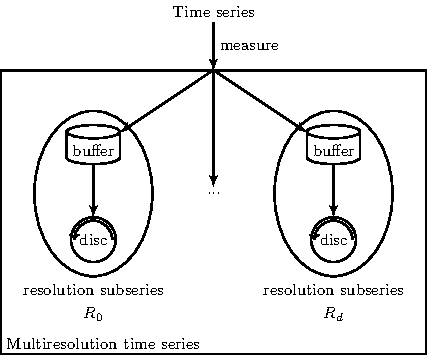
\includegraphics{fig_model_mtsdb.pdf}
  \caption{Architecture of \acro{MTSMS} model}
  \label{fig:model:mtsdb}
\end{figure}


In this way, the original time series gets stored spread in the discs,
each with a different time resolution and attribute aggregation.
Discs are size bounded so they only contain a fixed amount of
measures. When a disc becomes full it discards a measure. Thus,
multiresolution database is bounded in size and the time series gets
stored in pieces, that is time subseries.

Regarding operations, \acro{MTSMS} structure needs operators to change
the time intervals between measures and to select attributes. Mainly,
these operators are measure additions and time series consolidations,
which some functionality is delegated to operators called attribute
aggregate functions. Secondarily, there are operators to query the
multiresolution schema and extract time series data.


Following we define the \acro{MTSMS} model structure and structural
operators, the operations to query a multiresolution schema, and
attribute aggregate functions.  Furthermore, schema manipulation
operations could be defined but we focus on structure and data query .


\subsection{Structure}

A \emph{buffer} is a container for a regular or a no-regular time
series. The buffer objective is to regularise the time series using a
predetermined step and an attribute function. We name
\emph{consolidation} to this action.
\begin{definition}%(Buffer)
  A \emph{buffer} is defined as the tuple $(S_B,\tau,\delta,f)$ where
  $S_B$ is a time series, $\tau$ is the last consolidation time,
  $\delta$ is the duration of the consolidation step and $f$ is an
  attribute aggregate function.

  An empty buffer $B_{\emptyset} = (\emptyset,t_0, \delta, f)$ has an
  empty time series, an initial consolidation time $t_0$ and
  predetermined $\delta$ and $f$.
\end{definition}

Operator \emph{addBuffer} adds a measure to its time series:
$\addB: B = (S_B,\tau,\delta,f) \times m \mapsto
(S'_B,\tau,\delta,f)$ where $S'_B = S \cup \{m\} $.

From the $B_{\emptyset}$ all the consolidation time instants can be
calculated as $t_0+i\delta, i\in\N$. The consolidation of $B$ in a
time interval $i=[\tau,\tau+\delta]$ results in a measure
$m'=f(S_B,i)$ where $f$ is an attribute aggregate function
$f$. Operator \emph{consolidateBuffer} consolidates a set of measures
and removes the consolidated part of the time series from the buffer:
$\consB : B=(S_B,\tau,\delta,f) \mapsto B' \times m'$ where $ B'=
(S'_B,\tau+\delta,\delta,f)$, $m' = f(S,[\tau,\tau+\delta])$, and
$S'_B$ is the discarding of historic data not needed anymore, for example
$S'_B = S[\tau+\delta,+\infty]$.

On a simplified way, the \emph{consolidateBuffer} is only applied to the present
consolidation interval and the total consolidation is obtained by
successive application of the operator. This requires measures to be
added by time order and to consolidate the buffer when the time of
some measure is bigger than the buffer's next consolidation time.  Let
$B=(S_B,\tau,\delta,f)$ be a buffer and $m=\sup(S_B)$ the maximum
measure, $B$ is consolidable if and only if $T(m) \geq
\tau+\delta$.


A \emph{disc} is a finite capacity measures container. A time series
stored in a disc has its cardinal bounded. When the cardinal of the
time series is to overcome the limit, some measures need to be
discarded.
\begin{definition}%(Disc)
  A \emph{disc} is a tuple $(S_D,k)$ where $S_D$ is a time series and
  $k\in\N$ is the maximum allowed cardinal of $S_D$.  An empty disc
  $D_{\emptyset} = (\emptyset,k)$ has an empty time series and $k$ is
  the maximum cardinal allowed.
\end{definition}

The cardinal of the times series is kept under control by the add
operator, $\addD : D=(S_D,k)\times m\mapsto (S'_D,k)$ where %
$
 S_D' = \begin{cases}
  S_D\cup\{m\}                 & \text{if } |S_D|<k  \\
  (S_D-\{\min(S_D)\}) \cup \{m\} & \text{otherwise}
\end{cases}  
$.


A \emph{resolution subseries} is a structure that regularises and
aggregates a time series. It is composed of a buffer, that contains
the partial time series to be regularised, and a disc, that contains
the regularised time series.
\begin{definition}%(Resolution subseries)
  A \emph{resolution subseries} is a tuple $(B,D)$ where $B$ is a
  buffer and $D$ is a disc.  An empty buffer and empty disc imply an
  empty resolution subseries $R_{\emptyset} =
  (B_{\emptyset},D_{\emptyset})$.
\end{definition}
 
The operators of a resolution subseries extend the buffer and disc
ones: (i) The addition of a measure to the buffer of the resolution
subseries: $\addR : R=(B,D) \times m \mapsto R'$ where $R'= (B',D)$,
and $B'= \addB(B,m)$; (ii) The consolidation of the resolution
subseries by consolidating its buffer and adding the consolidation
measure to its disc: $\consR : R=(B,D) \mapsto R'$ where $R'=
(B',D')$, $(B',m') = \consB(B)$, and $D'= \addD(D,m')$.  A resolution
subseries is consolidable only when its buffer is consolidable.




A \emph{multiresolution time series} is a set of resolution subseries
which share the input of measures, that is the same time series. A
time series is stored regularised and distributed with different
resolutions in the various resolution subseries, as previously shown
in Figure~\ref{fig:model:mtsdb}.
\begin{definition}%(Multiresolution time series)
  A \emph{Mul\-ti\-re\-solution time series} is a set of resolution
  subseries $\{R_0, \dots, R_d\}$.  An empty multiresolution series
  has empty resolution subseries $M_{\emptyset}=\{R_{0_\emptyset},
  \dots, R_{d_\emptyset}\}$. Usually there are no repeated pairs of
  ($\delta_i$,$f_i$) among a multiresolution series, so they act as a
  key attributes.
\end{definition}

Therefore, defining a multiresolution time series consists basically
in defining the quantity of resolution subseries and the
$(\delta,\tau,f,k)$ configuration parameters of each.


The operators of a multiresolution time series apply to every
resolution subseries contained: (i) The addition of a measure to every
resolution subseries: $\addM : M=\{R_0,\allowbreak \dots,\allowbreak
R_d\} \times m \mapsto \{R'_0, \dots,\allowbreak R'_d\}$ where
$R'_i=\addR(R_i,m)$; (ii) The consolidation of all resolution
subseries: $\consM : M=\{R_0,\allowbreak \dots,\allowbreak R_d\}
\mapsto \{R'_0,\allowbreak \dots,\allowbreak R'_d\}$ where $R'_i =
\consR(R_i)$ if $R_i$ $\text{ consolidable}$ and $R'_i=R_i$
$\text{otherwise}$.


The multiresolution consolidation operation should be applied
regularly based on a consolidation clock. When the measure ordered
addition approach is taken as explained in the buffer's consolidation,
then there is no need for a clock in a \acro{MTSMS}. The consolidation clock
is induced by the measure's addition and then it is only necessary to
check the multiresolution consolidation operation on new
additions. However, there could be other approaches where the
consolidation clock was given by an external clock or external
events. Then the consolidable definitions would depend on this
external clock.





\subsection{Queries}


There are two basic time series queries for a \acro{MTSMS}: (i) extract a
time subseries from a resolution subseries' disc or (ii) query for a
total time series from all consolidated data.

The first is a selection of a disc over a multiresolution time series,
being $(\delta,f)$ the key attributes: $\seriedisc: M=\{R_0, \dots,
R_d\} \times \delta \times f \mapsto S'_D \in D' | (B',D') \in R',R' \in
M$.

The second is a concatenation of all discs' time subseries trying to
obtain the most resolution as possible, which is to say by $\delta$
order: $\totalseries: M*=\{R_0, \dots, R_d\} \mapsto S'$ where $S' =
S_{D0} || S_{D1} || \cdots || S_{Dd}$ and $\delta_0 < \delta_1 <
\cdots < \delta_d$. This states that $M*$ is a multiresolution time
subseries where $R_i$ have a total order by its attribute
$\delta_i$. Being $(\delta,f)$ the key attributes, the $M*$ can
be obtained from $M$ by selecting resolution subseries with same $f$. If we
operated a $\totalseries$ to a general $M$ then it could be ambiguous
as it could contain repeated $\delta_i$.


From these two basic time series queries, more elaborated queries can
be applied to \acro{MTSMS} by using \acro{TSMS} operations. For
example, let $M_1$ and $M_2$ be two multiresolution time series, we
can compute the sum of both with $\totalseries(M_1) +
\totalseries(M_2)$.
% This is the general algebraic expressions that describes the model,
% but an implementation of the model could accomplish this operation
% in a more efficient way.





\subsection{Attribute aggregate function}
\label{sec:model:interpolador}

Attribute aggregate functions are a specific case of \acro{TSMS}
aggregate operations for summarising time series data when
consolidating a buffer. Let $S$ be a time series and $t_0$ and $t_f$
two time instants, an attribute aggregate function $f$ calculates a
measure that summarises the measures of $S$ included in the time
interval $i=[t_0,t_f]$:
\[
f : S=\{m_0,\ldots,m_k\} \times i=[t_0,t_f] \mapsto m'
\]
where, generally, $m'$ results from two operations on the time series:
(i) a time subseries selection $S'$ depending on the consolidating
interval, for example $S' = S[t_0,t_f]$, and (ii) a \acro{TSMS} aggregation
over this time subseries such as $m' = \agg(S',m_i, f^a)$ where $f^a$
is a function over two measures.


Many different attribute aggregate functions can be used in order to
summarise a time series, for example it is possible to calculate an
statistic indicator of the time series such as the average or a more
complex digital signal processing operation
\cite{zhang11}. Furthermore, the representation for a time series and
some of its pathologies can be considered during the aggregation
process.


As it is possible to define many attribute aggregate
functions no global assumptions can be made about them. Each user has
to decide which combination of aggregation and representation fits
better with the measured phenomena.  Therefore, \acro{MTSMS} has to be
designed for allowing users to define aggregate functions.





Regarding the resulting consolidation time, normally it will be
$T(m')=t_f$ to be consistent with the consolidation operation of a
buffer where $\tau' = \tau + \delta \equiv t_f$. However $T(m')$ can
have a time offset with the buffer consolidating times, as instance
the resulting measure can be aggregated from a time subseries $S'$
with open interval $S'=S(t_0,t_f)$, closed interval $S'=S[t_0,t_f]$,
or other combinations like $S'=S(t_0-d,t_f-d]$ where $d$ is a time
duration.  The time offset can also be variable, as for example an
aggregate function that returns the first measure of the interval
$S[t_0,t_f)$, $m'=\min(S[t_0,t_f))$, then the resulting time can be
between $t_0 \leq T(m') < t_f$.


Attribute general patterns can be defined that explain how the
resulting value $V(m')$ is calculated, letting the resulting time
instant $T(m')$ subject to interpretation.  Next there are some
attribute patterns examples based on temporal function time series
operators, that is the time series aggregated corresponds to a
continuous function $S(t)^r$ where $r$ is a representation as has been
described in Section~\ref{sec:model:tfunc}. The patterns of these
functions leave $T(m')$ undefined as well as the representation $r$ of
the time series. Let the time be continuous on all the time domain
$t\in T$:
\begin{itemize}
\item maximum$^r$: $S \times i \mapsto m'$ where $V(m') =
  \max\limits_{\forall t \in i}(S(t)^r)$. It summarises $S$ with the maximum
  of the measure values in the interval $i$.
\item last$^r$: $S \times i \mapsto m'$ where $V(m') = S(t_f)^r$. It
  summarises $S$ with the value at $t_f$ time instant.
\item mean$^r$: $S \times i \mapsto m'$ where $V(m') =
  \frac{1}{t_f-t_0} \int\limits_{t_0}^{t_f} S(t)^r dt$. It summarises $S$
  with the mean of the function in the interval $i$.
\end{itemize}


These aggregation function patterns can be expressed with discrete
mathematics for each particular representation, that is based on the
temporal interval defined in Section~\ref{sec:model:tfunc}. Next we
exemplify it by interpreting the general continuous patterns for two
particular representations that have been defined previously: \dd{}
and \zohe{}.


Dirac delta attribute aggregation functions $f^\dd$ have a general
form $f^\dd : S \times [t_0,t_f]\mapsto m'$ where $m'=(t',v')$, the
resulting time is interpreted as centred on the interval
$t'=\frac{t_f+t_0}{2}$ and the resulting value depends on the
attribute, let $S'=S[t_0,t_f]^\dd$ be the selection of measures by
Dirac delta temporal interval:
\begin{itemize}
\item maximum$^\dd$: $v' = \max\big(0,\max_{\forall m \in S'}(V(m))\big)$. 
\item last$^\dd$: $v' = \max(S')$.
\item mean$^\dd$: $v' = \frac{1}{t_f-t_0} \sum\limits_{\forall m
    \in S'} V(m)$, as Dirac delta function has property $\int\dd(t)dt=1$.
\end{itemize}


\zohe{} attribute aggregation functions $f^\zohe{}$ have a general
form $f^\zohe{} : S \times [t_0,t_f]\mapsto m'$ where $m'=(t',v')$,
the resulting time is interpreted as right limit of the interval
$t'=t_f$ and the resulting value depends on the attribute, let
$S'=S[t_0,t_f]^\zohe{}$ be the selection of measures by \zohe{} temporal
interval:
\begin{itemize}
\item maximum$^\zohe{}$: $v' = \max_{\forall m \in S'}(V(m))$. 
\item last$^\zohe{}$: $v' = \max(S')$.
\item mean$^\zohe{}$: $v' = \frac{1}{t_f-t_0} \big[ (T(o)-t_0)V(o) +
  \sum\limits_{\forall m \in S''}( T(m)- T(\prev_S
  m) )V(m) \big]$ where $o=\min(S')$ and $S''= S' - \{o\}$.
\end{itemize}

A similar aggregation function to mean$^\zohe{}$ is used by \emph{RRDtool}
\cite{rrdtool} in order to summarise velocity coun\-ter
data by keeping the total counting information, as mean aggregation
can be seen as one keeping the area below the original signal.


In conclusion, some patterns are very similar. As instance maximum and
last attributes differ basically on the interval selection
operation. However, other patterns have a more elaborated
interpretation in a particular representation. As instance
mean$^\zohe{}$ and mean$^\dd$ are an elaborated interpretation for
the general integral definition.





\begin{example}\label{ex:model:smultiresolution} 
  We define a multiresolution schema for a time series, we consolidate
  the database and we query its data.  Let $S = \{
  (1,6),(5,2),\allowbreak (8,5),\allowbreak (10,0),\allowbreak
  (14,1),\allowbreak (19,6),\allowbreak (22,11),\allowbreak
  (26,6),(29,0) \}$ be a time series and $M_\emptyset=\{R_0,R_1\}$ a
  multiresolution time series where each resolution parameters are
  $\tau_0=0$ , $\delta_0=5$, $f_0 =\meanz$, $k_0=4$ and $\tau_1=0$,
  $\delta_1=10$, $f_1 =\maxz$, $k_1=2$. Therefore $R_0$ will be
  consolidated at time instants 5, 10, 15, 20, 25, 30\dots and $R_1$
  at 10, 20, 30\dots

  All measures of $S$ are added to $M_\emptyset$
  and then it is consolidated until it is no more consolidable. As
  $T(\max(S))=29$, the last consolidation times are $\tau_0=25$ and
  $\tau_1=20$, so we call $M_{29}$ to this multiresolution time series
  at this state.

  Then the two time subseries consolidated are obtained by querying
  $\seriedisc(M_{29},5,\allowbreak \meanz)=\{(10,3),\allowbreak
  (15,\allowbreak 2),\allowbreak (20,7),\allowbreak (25,8)\}$ and
  $\seriedisc(M_{29},10,\allowbreak  \maxz) =\allowbreak \{ \allowbreak
  (10,6),\allowbreak (20,11)\}$. Regarding buffers, note that
  $S_{B0_{29}}= \{\allowbreak (26,6),\allowbreak (29,0)\allowbreak \}$
  and $S_{B1_{29}}=\{\allowbreak (22,11),\allowbreak (26,6),(29,0)\}$.

  In this particular example
  $ \totalseries(M_{29}) = \seriedisc(M_{29},\allowbreak 5,\meanz)$ as $R_0$ has
  double resolution than $R_1$. $\square$
\end{example}



%%% Local Variables:
%%% TeX-master: "main"
%%% ispell-local-dictionary: "british"
%%% End:

% LocalWords:  genericity multiresolution subseries consolidable MTSM

% LocalWords:  pathologies MTSMS TSMS cardinality multivalued infimum
% LocalWords:  multivalues supremum
